\documentclass{tufte-handout}\usepackage[]{graphicx}\usepackage[]{xcolor}
% maxwidth is the original width if it is less than linewidth
% otherwise use linewidth (to make sure the graphics do not exceed the margin)
\makeatletter
\def\maxwidth{ %
  \ifdim\Gin@nat@width>\linewidth
    \linewidth
  \else
    \Gin@nat@width
  \fi
}
\makeatother

\definecolor{fgcolor}{rgb}{0.345, 0.345, 0.345}
\newcommand{\hlnum}[1]{\textcolor[rgb]{0.686,0.059,0.569}{#1}}%
\newcommand{\hlstr}[1]{\textcolor[rgb]{0.192,0.494,0.8}{#1}}%
\newcommand{\hlcom}[1]{\textcolor[rgb]{0.678,0.584,0.686}{\textit{#1}}}%
\newcommand{\hlopt}[1]{\textcolor[rgb]{0,0,0}{#1}}%
\newcommand{\hlstd}[1]{\textcolor[rgb]{0.345,0.345,0.345}{#1}}%
\newcommand{\hlkwa}[1]{\textcolor[rgb]{0.161,0.373,0.58}{\textbf{#1}}}%
\newcommand{\hlkwb}[1]{\textcolor[rgb]{0.69,0.353,0.396}{#1}}%
\newcommand{\hlkwc}[1]{\textcolor[rgb]{0.333,0.667,0.333}{#1}}%
\newcommand{\hlkwd}[1]{\textcolor[rgb]{0.737,0.353,0.396}{\textbf{#1}}}%
\let\hlipl\hlkwb

\usepackage{framed}
\makeatletter
\newenvironment{kframe}{%
 \def\at@end@of@kframe{}%
 \ifinner\ifhmode%
  \def\at@end@of@kframe{\end{minipage}}%
  \begin{minipage}{\columnwidth}%
 \fi\fi%
 \def\FrameCommand##1{\hskip\@totalleftmargin \hskip-\fboxsep
 \colorbox{shadecolor}{##1}\hskip-\fboxsep
     % There is no \\@totalrightmargin, so:
     \hskip-\linewidth \hskip-\@totalleftmargin \hskip\columnwidth}%
 \MakeFramed {\advance\hsize-\width
   \@totalleftmargin\z@ \linewidth\hsize
   \@setminipage}}%
 {\par\unskip\endMakeFramed%
 \at@end@of@kframe}
\makeatother

\definecolor{shadecolor}{rgb}{.97, .97, .97}
\definecolor{messagecolor}{rgb}{0, 0, 0}
\definecolor{warningcolor}{rgb}{1, 0, 1}
\definecolor{errorcolor}{rgb}{1, 0, 0}
\newenvironment{knitrout}{}{} % an empty environment to be redefined in TeX

\usepackage{alltt}

%\geometry{showframe}% for debugging purposes -- displays the margins

\usepackage{amsmath}
\usepackage{graphicx}
\usepackage{natbib}
\usepackage{cancel}
\usepackage{comment}

\setkeys{Gin}{width=\linewidth,totalheight=\textheight,keepaspectratio}
\bibfont{\small} % Doesn't see to work...

\graphicspath{{graphics/}}

\newenvironment{itemize*}%
  {\begin{itemize}%
    \setlength{\itemsep}{0pt}%
    \setlength{\parskip}{0pt}}%
  {\end{itemize}}
	
\newenvironment{enumerate*}%
  {\begin{enumerate}%
    \setlength{\itemsep}{0pt}%
    \setlength{\parskip}{0pt}}%
  {\end{enumerate}}
	
	\newenvironment{description*}%
  {\begin{description}%
    \setlength{\itemsep}{0pt}%
    \setlength{\parskip}{0pt}}%
  {\end{description}}

\newcommand{\numolspercm}{$\mu$mols/cm$^{-3}$}

\title{DRAFT! Advection, Diffusion \& Reaction Modeling}
\author{Marc Los Huertos}
\date{\today~(ver.~0.85)}

\setsidenotefont{\color{blue}}
% \setcaptionfont{hfont commandsi}
% \setmarginnotefont{\color{blue}}
% \setcitationfont{\color{gray}}

% The following package makes prettier tables.  We're all about the bling!
\usepackage{booktabs}

% Small sections of multiple columns
\usepackage{multicol}
\IfFileExists{upquote.sty}{\usepackage{upquote}}{}
\begin{document}

\maketitle% this prints the handout title, author, and date
\sidenote{Document progress: This is a draft document that will be used to help Marc develop some code with Ami in Math. Unitl the version reaches 1.0, consider this a non-functional draft.}


\begin{abstract}
The movement of compounds in the environment is driven by two processes, advection and diffusion. The compounds are also subject to transformations or reactions. Thus, to monitor the fate and transport of compounds in the environment, we can capitalize on mathematical models that have been used to describe advection, diffusion, and reaction. %We'll begin with simple examples and then consider more complicated examples. We'll also consider the implications of these processes on the environment and human health.

%\sidenote{Typeset using the Sweave function in R and \LaTeX\ using a \citet{Tufte:1983, Tufte:1997} and style.}
\end{abstract}



\section{Introduction}

\subsection{Fate and Transport Processes}

The fate and transport of compounds in the environment is subject to an array of processes. For example, pollutants might carried by the wind (advection) and spread out (dispersion or diffusion). In addition, the pollutant might be transformed into different compounds (reaction). Together, these three processes, advection, diffusion, and reaction (Figure~\ref{fig:advection-diffusion}).%, can be effectively described mathematically, which can then be tested.

%. Of course, these processes occur in three dimensions but we'll focus on 1D and 2D for this session. 

\begin{marginfigure}
\centering
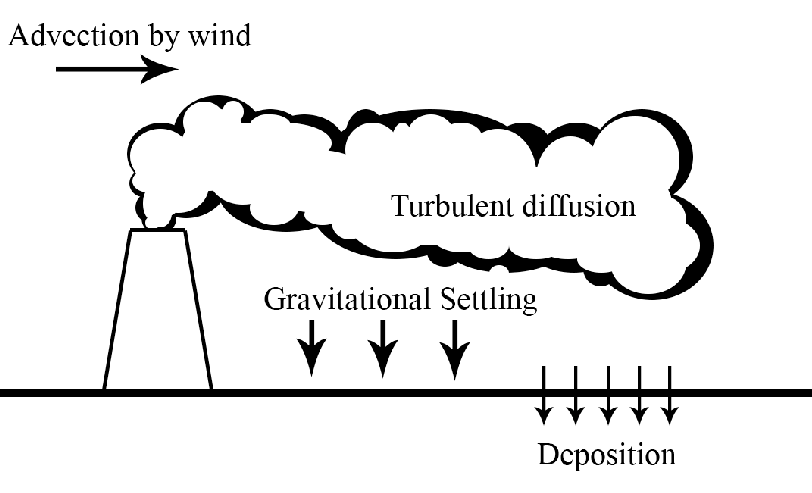
\includegraphics[width=1.0\textwidth]{graphics/Diagram-advection-diffusion.png}
\caption{A simple diagram of advection and diffusion that inclues how "solutes" might be deposited downwind of a stationary source if air pollution. At the scale analyzed there, the term turbulant diffusion is different than molecular diffusion, but might be modelled in a similar way.}
\label{fig:advection-diffusion}
\end{marginfigure}


These three processes have profound  implications -- they provide the a framework to understand and quantify the fate and transport of pollutants in the environment (Figure~\ref{fig:dioxaneplume}), the movement of nutrients in the soil, and the movement of solutes in the human body. By understanding of these processes, we have tools to characterize environmental quality and its implications on human and non-human populations. Moreover, by modeling these processes, we can develop more effective policy, regulation, and mitigation strategies.

\begin{figure*}
\centering
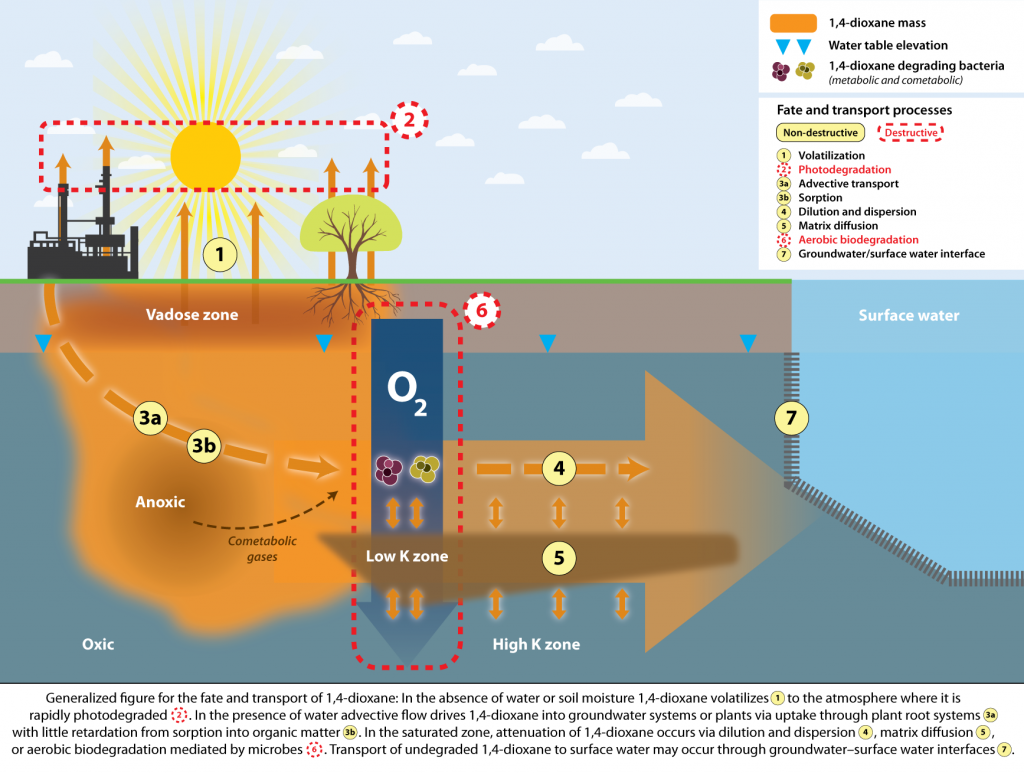
\includegraphics[width=0.9\textwidth]{graphics/Dioxane_plume.png}
\caption{A diagram of the major processes that influence the fate and transport of a dioxane plume from a ce in the environment (Source: \url{https://14d-1.itrcweb.org/environmental-fate-transport-and-investigative-strategies/}). 1,4-Dioxane is often referred to as a "forever" compound.}
\label{fig:dioxaneplume}
\end{figure*}

Because these processes are complex and are often difficult to measure, we rely on models to help us understand the movement of solutes in the environment. These models are based on the fundamental mathematical equations to describe advection, diffusion, and reaction.

\subsection{The Processes}

As an example of the three processes consider a droplet of dye in water as a dose in a solution. The dye will move with the bulk motion of the water (advection), spread out by random molecular motion (diffusion)(Figure~\ref{fig:diffusion}), and disappear as it reacts with the water (reaction).

Advection and diffusion govern the transport of solutes in the environment. Advection is the transport of a solute by the bulk motion of the fluid. Advection depends on velocity or $\nu$ in this session. Diffusion is the transport of a solute by random molecular motion. Diffusion depends on the diffusion coefficient and the concentration gradient or $\frac{\partial^2 C}{\partial x^2}$ in this session. Notice that this is the second derivative. 

\begin{marginfigure}
\caption{A simple diagram of 2D diffusion. To solve these equations, we'll use a numerical approach and descretize the media into a grid. We'll then solve the equations for each grid cell.}
\label{fig:diffusion}
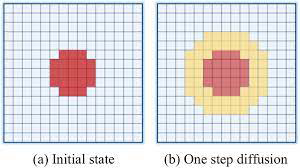
\includegraphics[width=1.0\textwidth]{graphics/2D_diffusion.png}
\end{marginfigure}

Reaction is the transformation of a solute into a different compound. Reaction depends on the reaction rate or $k$ in this session.

In the case of air pollution, we are interested in the pollutant in the context of the air -- or the media of air (Figure~\ref{fig:advection-diffusion}). And for air pollution, the chemical transormations are a critical part of our regulatory framework (Figure~\ref{}). In the case of water, we might think about solutes in the water as a media. For example, the movement of a nutrient in a river is driven by the bulk motion of the water (advection) through the water column and the sediments (two types of media) and the random motion of the molecules (diffusion) and the reactions that might occur in the water column and sediments (Figure\ref{fig:nutrientspiraling}).

\begin{figure*}
\caption{A simple diagram of advection and diffusion in the context of air pollution.}
\label{fig:smog}
\centering
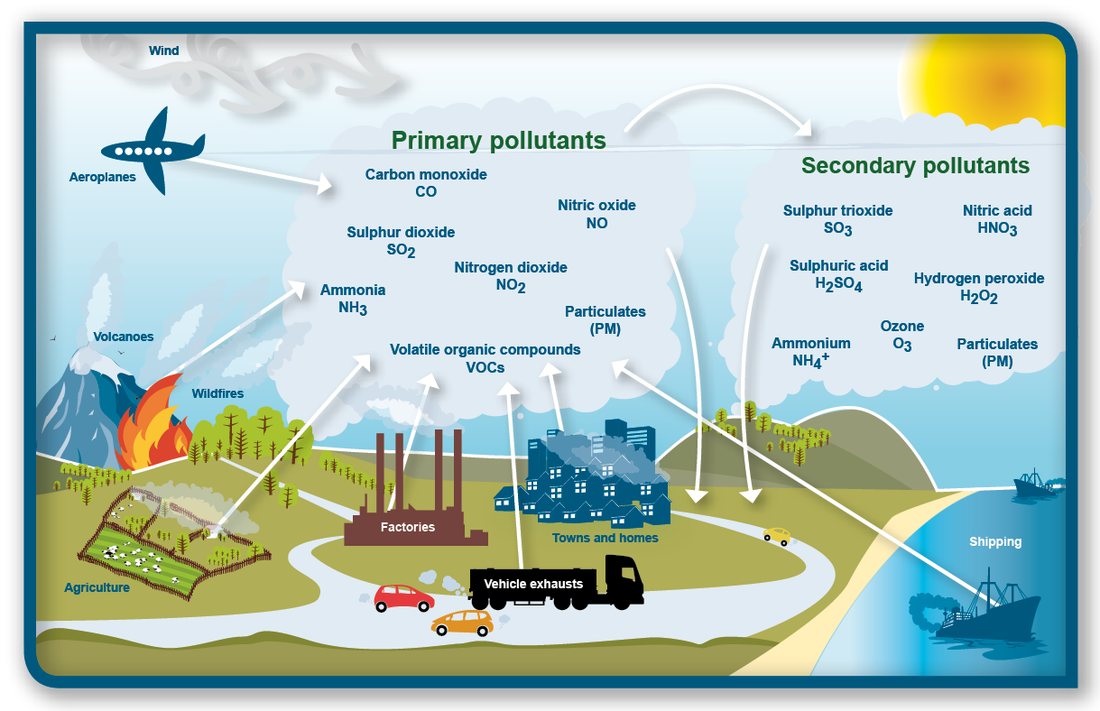
\includegraphics[width=0.99\textwidth]{graphics/sources-of-air-pollution-310314_orig.png}
\end{figure*}


\begin{figure}
\caption{A simple diagram of advection and nutrient reactions (organic substances and inorganic substances) in a river. Although not shown, you might also think about how diffusion might influence the movement of nutrients in the river and in the sediments.  
The zone where water moves into the sediment bed is called the hyperreic zone. The porosity of the sediments will allow more advective flow that might influence the reaction capacity of solutes in the sediments.}
\label{fig:nutrientspiraling}
\centering
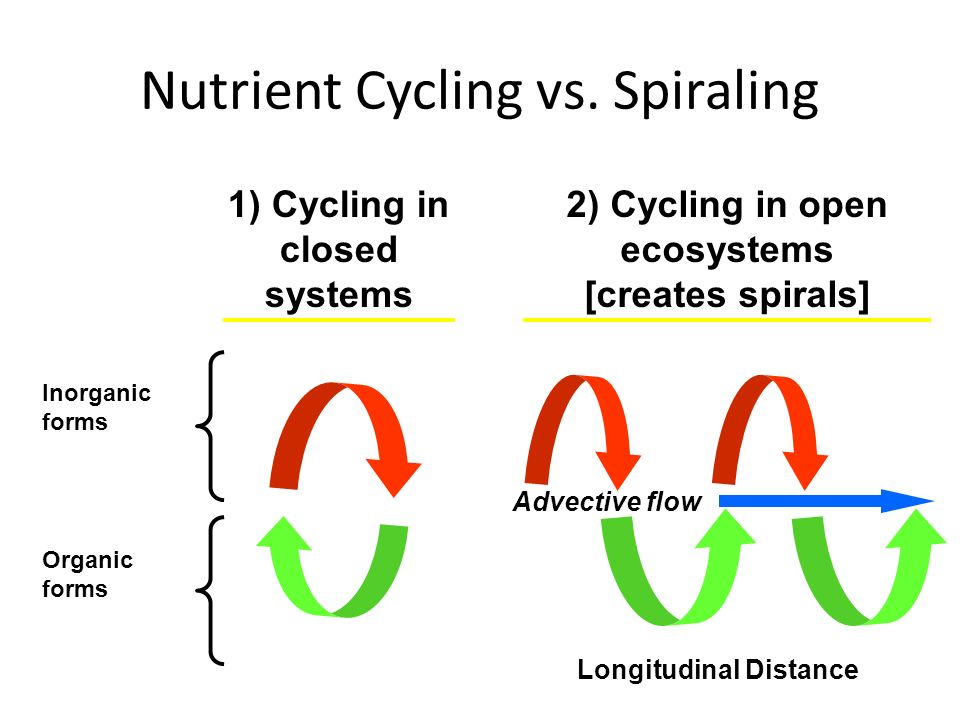
\includegraphics[width=0.99\textwidth]{graphics/NutrientSpiraling.jpg}
\end{figure}
jk
\subsection{Session Goals}

We will not become experts in advection-diffusion-reaction modeling, but we will become familiar with the processes and the equations that describe them. Moreover, we'll see a bit more about how R can be used to model these processes. After this session, I hope you can do the following:

\begin{enumerate*}
	\item Describe the physical processes of advection and diffusion and solute reaction
	\item Describe the equations used to model A-D-R. 
	\item Analyze 1-dimensional movement using advection equations in R.
	\item Describe diffusion mathematically
	\item Analyze 1-dimensional adveecton-diffusion using R.
	\item Appreciate how two-dimensional analysis of advection-diffusion can be modeled in R.
\end{enumerate*}

In this session, we'll want to think about the movement of solutes in the porous media, i.e. a soil with air space, sediments with water between the particles. We will refer to the porousity as $\xi$, which is a proportion between 0 and 1. 

\begin{marginfigure}
\centering
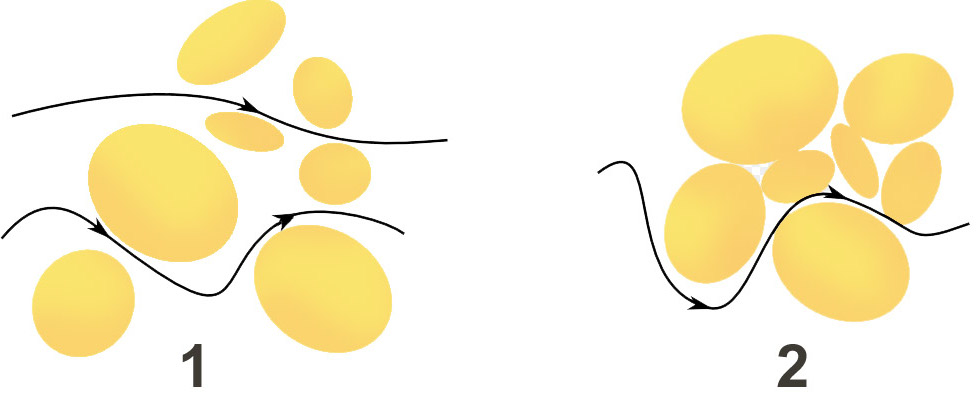
\includegraphics{graphics/Darcy_permeability.jpg}
\caption{Notice how the porosity of the media can influence the path of the fluid. In ground water, this is measured as permeability and can be used to evaluate the flow chacterstitics in aquifers and oil fields. The permeability is a function of the porosity and the connectivity of the pores.}
\end{marginfigure}

%We'll start with one-dimensional systems and then move to two-dimensional systems. We'll also consider the effects of reactions on the movement of solutes.

\section{Equations to Describe Processes}

\newthought{An Equation that Often Creates Anxiety}

The advection equation is a partial differential equation that describes the movement of a substance in a fluid. The equation is derived from the conservation of mass. The equation is:

%− 1 Axξx ·( ∂ ∂xAx·(−D· ∂ξxC ∂x )− ∂ ∂x(Ax·v·ξxC)) 

%\begin{equation}
%- \frac{1}{A_x \xi_x} \cdot \left( \frac{\partial}{\partial x} A_x \cdot \left( -D \cdot %\frac{\partial \xi_x C}{\partial x} \right) - \frac{\partial}{\partial x} \left( A_x \cdot v \cdot \xi_x C \right) \right)
%\end{equation}

\begin{equation}
\frac{\partial C}{\partial t} = D_x \frac{\partial^2  \xi_x C}{\partial x^2} +
D_y \frac{\partial^2  \xi_y C}{\partial y^2} +
D_z \frac{\partial^2  \xi_z C}{\partial z^2} -
v_x \frac{\partial  \xi_x C}{\partial x} - R
\end{equation}

Here $D$ is the ``diffusion coefficient'', $\nu$ is the ``advection rate'' (or velocity), and $A_x$ and $\xi$ are the surface area and volume fraction, respectively.

As you complete the first part of this handout, please do some reflecting: 

\begin{quote}

What you look at this equation, think about how it makes you feel. It's a bit intimidating, to say the least. But that's only part of the story. I believe these equations, when put in front of is generates anxiety -- and this anxiety can be a barrier to learning. While it's easy to claim we can just put this anxiety away seems to be be a disservice and acknoweldgement of our emotional responses. Before moving forward, let's take a moment to acknowledge the anxiety and see where in your body you are feeling that. Take a deep breath and let it out several times before moving forward.

\end{quote} 

First, let's simplify this to 1-D (in one direction, x). And assume that the volume fraction is 1 ($xi = 1$). The movement of compounds in the environment is driven by two processes, advection and diffusion -- these terms associated with $\partial x$ define movement. The third term on the right, $R$, is the reaction term.

\begin{equation}
\frac{\partial C}{\partial t} = D \frac{\partial^2 C}{\partial x^2} - \nu \frac{\partial C}{\partial x} - R
\end{equation}

\subsection{Left side: $\frac{\partial C}{\partial t}$}

The left side of the equation describes the change in concentration over time. This is the rate of change of the concentration of the solute in the fluid. In steady state, this term is zero, which will use use to model the steady state concentration of the solute in the fluid.

\subsection{First term on the right side: $D \frac{\partial^2 C}{\partial x^2}$}

The first term on the right side of the equation describes the movement of the solute due to diffusion. This is the rate of change of the concentration of the solute in the fluid due to the movement of the solute from areas of high concentration to areas of low concentration.

\subsection{Second term on the right side: $- \nu \frac{\partial C}{\partial x}$}

The second term on the right side of the equation describes the movement of the solute due to advection. This is the rate of change of the concentration of the solute in the fluid due to the movement of the fluid.

\subsection{Third term on the right side: $- R$}

The third term on the right side of the equation describes the rate of change of the concentration of the solute in the fluid due to reactions. This is the rate of change of the concentration of the solute in the fluid due to the reaction of the solute with other compounds in the fluid.

\begin{quote}
\textbf{Pause for a moment:} Reflect on your emotional state. What are you feeling? Where are you feeling it? Take a deep breath and let it out several times. You have completed the reading for Wednesday's class. 
\end{quote}

\section{2/21 Handout Update}



\section{Quatifying Advective Transport}

\begin{equation}
  J = C \cdot \nu
\end{equation}

J is the ``flux density'' of the solute, which is the amount of solute that moves through a unit area in a unit time. With units of $mass / (area \cdot time)$, the equation returns the rate of movement of the solute in the fluid.


We can take the derivative of the flux density with respect to the distance to get the ``flux rate'' and then derive the concentration change with respect to time: \sidenote{How dows J become C??}

\begin{equation}
  \frac{\partial J}{\partial x} = \nu \frac{\partial C}{\partial t}
\end{equation}


of the solute, which is the amount of solute that moves through a unit area in a unit time. With units of $mass / (area \cdot time)$, the equation returns the rate of movement of the solute in the fluid.

\section{Diffusion}

\subsection{Fick's First Law and Three Types of Diffusion}

There are three types of diffusion: turbulent (eddy) diffusion, dispersion and molecular diffusion. Each of the operate at different scales, but have similar effects and are describe by the same equation:

\begin{equation}\label{eq:ficks-first-law}
  J = -D \frac{d C}{dx}
\end{equation}

Equation~\ref{eq:ficks-first-law} ss known as Fick's first law. The negative sign indicates that the solute moves from areas of high concentration to areas of low concentration. The equation returns the rate of movement of the solute in the fluid.

\begin{description*}

\item[Turbulent or Eddy diffusion] is the movement of solutes due to the movement of the fluid. In this case, D is the ``eddy diffusion coefficient''.

\item[Dispersion] is the movement of solutes due to the random movement of the solute through a porous media where D is the ``dispersion coefficient''.

\item[Molecular diffusion] is the movement of solutes due to the random movement of the solute molecules where D is the ``molecular diffusion coefficient''.

\end{description*}

\subsection{Fick's Second Law -- Rate of Change}

STILL WORKING ON THIS... 

Fick's Second Law is based on the conservation of mass, where the rate of change of the concentration of the solute in the fluid due to the movement of the solute from areas of high concentration to areas of low concentration is described by the equation:

\begin{equation}
  \frac{\partial C}{\partial t} + \frac{\partial}{\partial x} J = 0 \rightarrow  \frac{\partial C}{\partial t} = - \frac{\partial}{\partial x}( D \frac{\partial}{\partial x} C) = 0
\end{equation}

\begin{equation}
  \frac{\partial C}{\partial t} = D \frac{\partial^2 C}{\partial x^2}
\end{equation}

which can be written as 

\begin{equation}
  \frac{\partial C}{\partial t} + D \frac{\partial^2 C}{\partial x^2} = 0
\end{equation}



We can rearrange Fick's first law to get the rate of change of the concentration of the solute in the fluid due to the movement of the solute from areas of high concentration to areas of low concentration:

\begin{equation}
  \frac{\partial C}{\partial t} + D \frac{\partial^2 C}{\partial x^2}
\end{equation}


Based on the conservation of mass, we can derive the rate of change of the concentration of the solute in the fluid due to the movement of the solute from areas of high concentration to areas of low concentration:


\begin{equation}
  \frac{\partial C}{\partial t} = D \frac{\partial^2 C}{\partial x^2}
\end{equation}

This equation is known as Fick's second law. It describes the rate of change of the concentration of the solute in the fluid due to the movement of the solute from areas of high concentration to areas of low concentration.

\section{Applications using R}

\subsection{ReacTran Package}

\citet{soetaert2017package} have developed a nice library in R that solves these equations using finite-difference solutions. 

The ReacTran package is a collection of functions for modeling solute transport in 1D, 2D, and 3D. The package includes functions for solving the advection-diffusion equation, the advection-diffusion-reaction equation, and the advection-diffusion-reaction equation for multi-phase systems. 

The package also includes functions for solving:

\begin{itemize*}
\item Advection-diffusion equations in 1D, 2D, and 3D 
\item Advection-diffusion-reaction equations in 1D, 2D, and 3D
\item Advection-diffusion-reaction equations for multi-phase systems
\end{itemize*}

\subsection{Using R as a Modelling Environment to Solve PDEs and ODEs}

We can use R to solve the advection-diffusion equation. The `deSolve` package to solve the ReacTran library functions decomposing the partial differential equatation (PDE) into a descretized by space and solving be ordinary differential equations (ODE). 

\begin{knitrout}
\definecolor{shadecolor}{rgb}{0.969, 0.969, 0.969}\color{fgcolor}\begin{kframe}
\begin{alltt}
\hlkwd{library}\hlstd{(ReacTran)} \hlcom{# Load the ReacTran package}
\end{alltt}


{\ttfamily\noindent\itshape\color{messagecolor}{\#\# Loading required package: rootSolve}}

{\ttfamily\noindent\itshape\color{messagecolor}{\#\# Loading required package: deSolve}}

{\ttfamily\noindent\itshape\color{messagecolor}{\#\# Loading required package: shape}}\begin{alltt}
\hlkwd{library}\hlstd{(deSolve)} \hlcom{# Load the deSolve package}
\hlkwd{library}\hlstd{(xtable)} \hlcom{# Load the xtable package to help format tables outputs}
\end{alltt}
\end{kframe}
\end{knitrout}

Much of the complexity for modeling solute transport in 1D, 2D, and 3D is in the boundary conditions, initial conditions, and the rate of reaction. If these are not carefully considered, the model, which is an interative process, may not ``converge'' to a solution.

\subsection{Grid and Time Step}

Setting up the grid and time step is the first step in solving the advection-diffusion equation. The grid is the spatial domain over which the solute is transported, and the time step is the time domain over which the solute is transported. The grid and time step are used to discretize the advection-diffusion equation, which is a partial differential equation that describes the rate of change of the concentration of the solute in the fluid due to the movement of the solute from areas of high concentration to areas of low concentration.

Here are some rules of thumb for setting up the grid and time step:

\begin{itemize*}
\item The grid should be fine enough to capture the spatial variation of the solute in the fluid.

\noindent General equation??

\item The time step should be small enough to capture the temporal variation of the solute in the fluid.

\noindent General equation??

\end{itemize*}



\subsection{Steady-state vs. Transient State}

The advection-diffusion equation can be solved in either the steady-state or transient state. 

The steady-state solution is used to determine the concentration of the solute in the fluid at a given time, while the transient state solution is used to determine the concentration of the solute in the fluid over time.

\subsection{Boundary Conditions}

The boundary conditions are used to specify the concentration of the solute in the fluid at the boundaries of the grid. The boundary conditions are used to specify the concentration of the solute in the fluid at the inlet and outlet of the grid, and at the top and bottom of the grid.

\subsection{Initial Conditions}

The initial conditions are used to specify the concentration of the solute in the fluid at the start of the simulation. The initial conditions are used to specify the concentration of the solute in the fluid at the start of the simulation, and at the start of each time step.



\subsection{Rate of Reaction}



\begin{verbatim}
parms <- c(v = v, D = D, dx = dx, nx = nx)

C <- ode(y = C, times = t, func = solute_transport, parms = parms)
\end{verbatim}


\section{Implemeting Some 1D Examples in R}

\subsection{Plug Flow  -- Salts in a River}

\subsection{Pulse Injection -- Tracer Test}

Tracer test are used to determine the flow velocity of a fluid. The tracer is injected into the fluid and the concentration of the tracer is measured at a downstream location. The time it takes for the tracer to travel from the injection point to the downstream location is used to determine the flow velocity of the fluid.

The advection-dispersion model is used to predict the concentration of the tracer at the downstream location. The model is based on the advection-diffusion equation, which describes the movement of the tracer through the fluid. The advection-dispersion model is a partial differential equation that describes the rate of change of the concentration of the tracer in the fluid due to the movement of the tracer from areas of high concentration to areas of low concentration.

The advection-dispersion model is based on the conservation of mass, where the rate of change of the concentration of the tracer in the fluid due to the movement of the tracer from areas of high concentration to areas of low concentration is described by the equation:

\begin{equation}
  \frac{\partial C}{\partial t} + \frac{\partial}{\partial x} J = 0 \rightarrow  \frac{\partial C}{\partial t} = - \frac{\partial}{\partial x}( D \frac{\partial}{\partial x} C) = 0
\end{equation}

\begin{knitrout}
\definecolor{shadecolor}{rgb}{0.969, 0.969, 0.969}\color{fgcolor}\begin{kframe}
\begin{alltt}
\hlcom{# pulse tracer test in water without decay}
\hlcom{# simple diffusion portion?? not sure where...}
\hlstd{pulseTracer} \hlkwb{<-} \hlkwa{function}\hlstd{(}\hlkwc{x}\hlstd{,} \hlkwc{t}\hlstd{,} \hlkwc{D}\hlstd{,} \hlkwc{v}\hlstd{,} \hlkwc{C0}\hlstd{) \{}
  \hlstd{C} \hlkwb{<-} \hlstd{C0} \hlopt{*} \hlkwd{exp}\hlstd{(}\hlopt{-}\hlstd{v} \hlopt{*} \hlstd{x} \hlopt{/} \hlstd{D)} \hlopt{/} \hlkwd{sqrt}\hlstd{(}\hlnum{4} \hlopt{*} \hlstd{pi} \hlopt{*} \hlstd{D} \hlopt{*} \hlstd{t)}
  \hlkwd{return}\hlstd{(C)}
\hlstd{\}}

\hlcom{# Solve}
\hlstd{x} \hlkwb{<-} \hlkwd{seq}\hlstd{(}\hlnum{0}\hlstd{,} \hlnum{6}\hlstd{,} \hlnum{.1}\hlstd{)}
\hlstd{t} \hlkwb{<-} \hlnum{1}
\hlstd{D} \hlkwb{<-} \hlnum{1}
\hlstd{v} \hlkwb{<-} \hlnum{1}
\hlstd{C0} \hlkwb{<-} \hlnum{1}



\hlstd{C} \hlkwb{<-} \hlkwd{pulseTracer}\hlstd{(x, t, D, v, C0)}
\hlkwd{plot}\hlstd{(x, C,} \hlkwc{type} \hlstd{=} \hlstr{"l"}\hlstd{,} \hlkwc{xlab} \hlstd{=} \hlstr{"Distance"}\hlstd{,} \hlkwc{ylab} \hlstd{=} \hlstr{"Concentration"}\hlstd{,} \hlkwc{main} \hlstd{=} \hlstr{"Pulse Tracer Test"}\hlstd{,} \hlkwc{ylim}\hlstd{=}\hlkwd{c}\hlstd{(}\hlnum{0}\hlstd{,} \hlnum{0.4}\hlstd{))}
\hlkwa{for}\hlstd{(t} \hlkwa{in} \hlkwd{seq}\hlstd{(}\hlnum{1}\hlstd{,} \hlnum{10}\hlstd{,} \hlnum{1}\hlstd{)) \{}
  \hlstd{C} \hlkwb{<-} \hlkwd{pulseTracer}\hlstd{(x, t, D, v, C0)}
  \hlkwd{lines}\hlstd{(x, C,} \hlkwc{col} \hlstd{= t)}
\hlstd{\}}
\end{alltt}
\end{kframe}
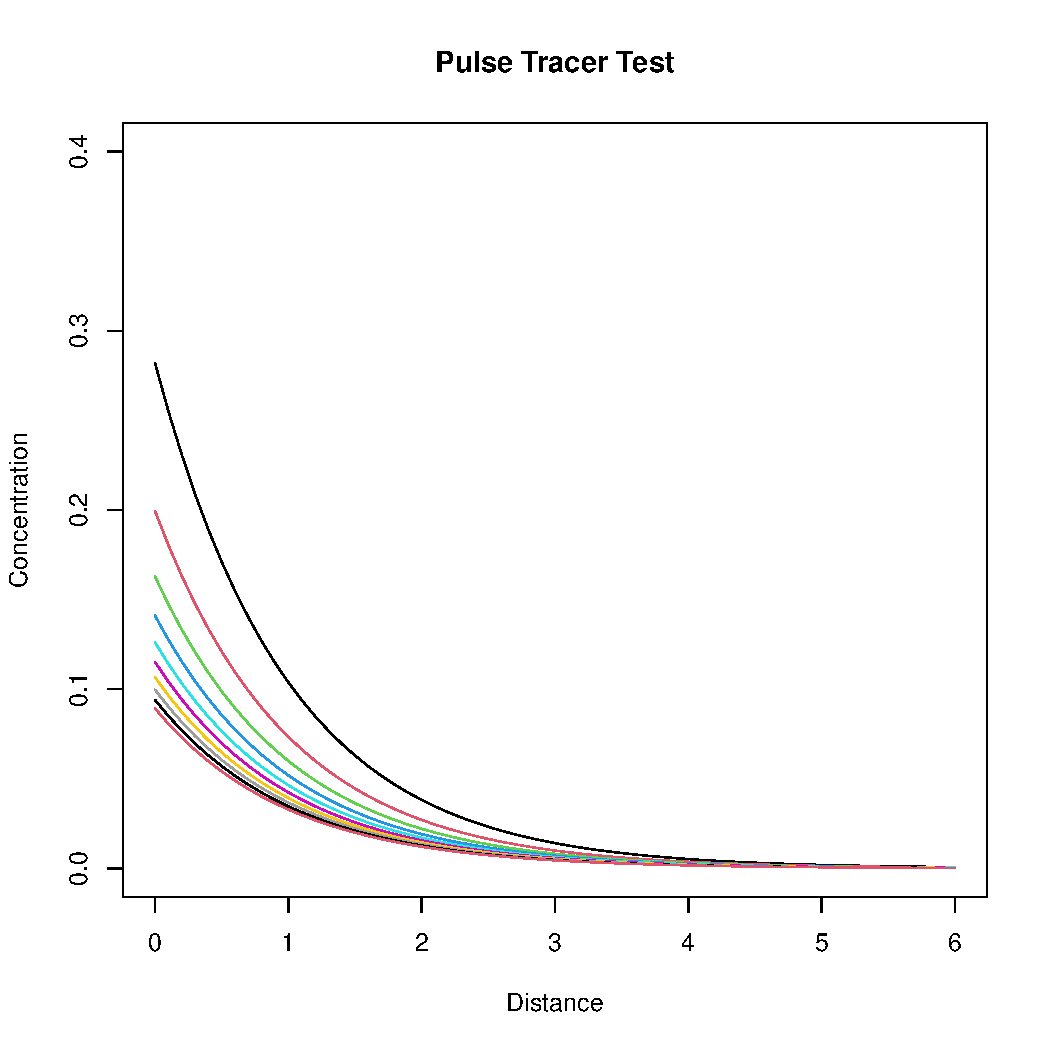
\includegraphics[width=\maxwidth]{figure/unnamed-chunk-2-1} 
\end{knitrout}

\subsection{Pulse Injection -- Tracer Test with Decay}


The impacts of matrix diffusion on the initial breakthrough of the solute plume and on later cleanup are illustrated in Figure~\ref{fig:ADRFig3}). 

\begin{marginfigure}
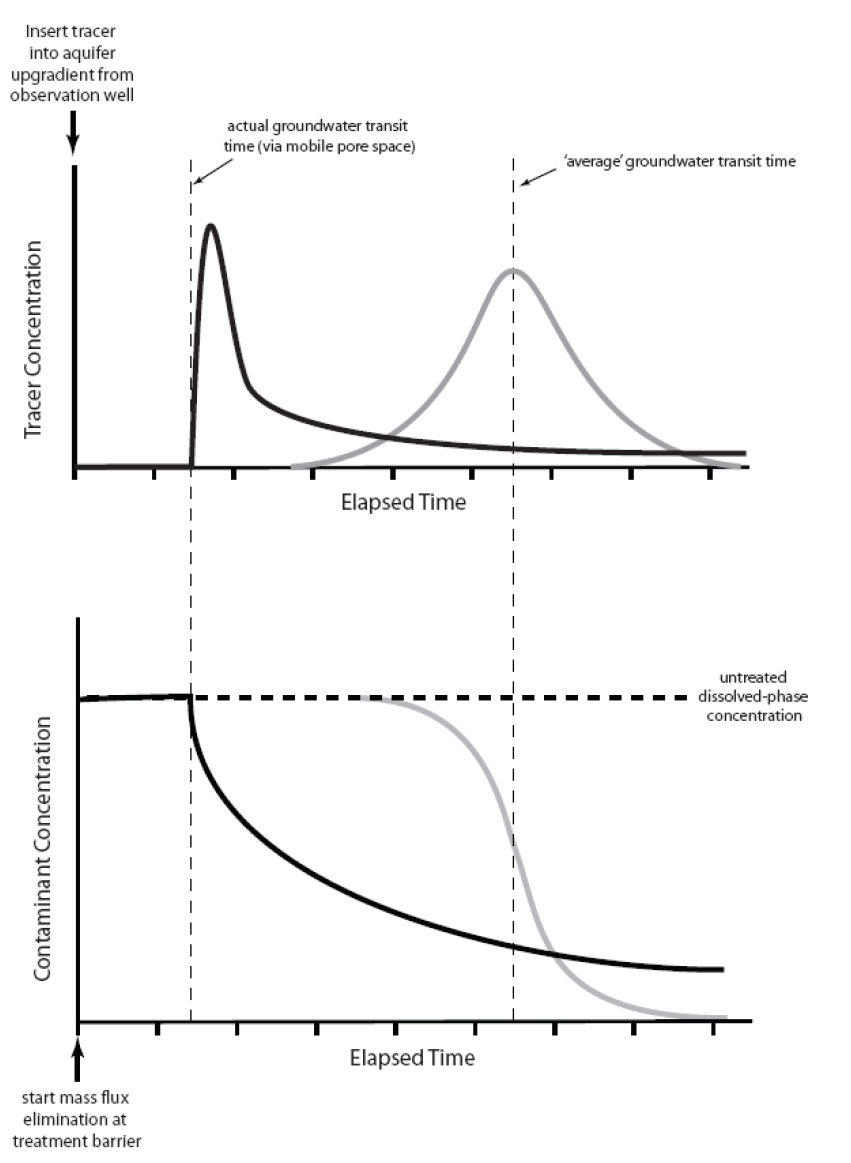
\includegraphics[width=1.0\textwidth]{graphics/ADRFig3.png}
\caption{Using a traditional advection-dispersion model, the breakthrough curve for a pulse tracer injection appears as a bell-shaped (Gaussian) curve (gray line on the right side of the upper graph) where the peak arrival time corresponds to the average groundwater velocity. Using an advection-diffusion approach, the breakthrough curve for a pulse injection is asymmetric (solid black line) with the peak tracer concentration arriving earlier than would be expected based on the average groundwater velocity, but with a long extended tail to the flushout curve.}
\label{fig:ADRFig3}
\end{marginfigure}

The lower graph in Figure~\ref{fig:ADRFig3} shows the predicted cleanup concentration profiles following complete elimination of a source area. The advection-dispersion model (gray line) predicts a clean-water front arriving at a time corresponding to the average groundwater velocity. The advection-diffusion model (black line) predicts that concentrations will start to decline more rapidly than expected (based on the average groundwater velocity) as clean water rapidly migrates through the highest-permeability strata. However, low but significant contaminant concentrations linger much longer (tailing) due to diffusive contaminant mass exchange between zones of high and low permeability.

\begin{equation}
\frac{d C\nu_vc}{d t} = \Sigma Q_{in} \cdot C_{in} - \Sigma Q_{out} \cdot C_{out} + \Sigma R V_{cv}
\end{equation}


\begin{equation}
  \frac{\partial C}{\partial t} = - \nu \frac{\partial C}{\partial x}
\end{equation}

\begin{equation}
C(x,t) = \frac{M}{A \sqrt{4\pi D_d t}} \cdot \exp[\frac{−x^{\prime 2}}{4D_d t}]
\end{equation}

Where:\\
M = mass of conservative material in the spike\\
Dd = axial dispersion coefficient [L2/T],\\
x’ = x - Ut, U = longitudinal advective velocity in the reactor,\\
A is the cross-sectional area of the reactor.\\

First we make a one-dimensional grid and define the parameters of the problem.\sidenote{The future code is going to rely on ReacTran package.}

\begin{knitrout}
\definecolor{shadecolor}{rgb}{0.969, 0.969, 0.969}\color{fgcolor}\begin{kframe}
\begin{alltt}
\hlcom{# working on this}

\hlstd{L} \hlkwb{<-} \hlnum{1} \hlcom{# length of the grid, 10 meters}
\hlstd{nx} \hlkwb{<-} \hlnum{100} \hlcom{# number of grid cells}
\hlstd{dx} \hlkwb{<-} \hlstd{L}\hlopt{/}\hlstd{nx} \hlcom{# length of each grid cell}
\hlstd{x} \hlkwb{<-} \hlkwd{seq}\hlstd{(}\hlnum{0}\hlstd{, L,} \hlkwc{by}\hlstd{=dx)} \hlcom{# grid}
\hlstd{D} \hlkwb{<-} \hlnum{0.1} \hlcom{# diffusion coefficient}
\end{alltt}
\end{kframe}
\end{knitrout}

Next, we define the initial and boundary conditions. We will assume that the concentration of the solute is zero at the beginning of the experiment and that the concentration of the solute is constant at the boundaries of the grid.

\begin{knitrout}
\definecolor{shadecolor}{rgb}{0.969, 0.969, 0.969}\color{fgcolor}\begin{kframe}
\begin{alltt}
\hlcom{# working on this}

\hlstd{v} \hlkwb{<-} \hlnum{0.1} \hlcom{# advection velocity}
\hlstd{t} \hlkwb{<-} \hlnum{0.1} \hlcom{# times}
\hlstd{C} \hlkwb{<-} \hlnum{0} \hlcom{# concentration of the solute}
\end{alltt}
\end{kframe}
\end{knitrout}

Next we define the functions that will be used to solve the advection-diffusion equation.

\begin{knitrout}
\definecolor{shadecolor}{rgb}{0.969, 0.969, 0.969}\color{fgcolor}\begin{kframe}
\begin{alltt}
\hlcom{# working on this}
\hlcom{# define the solute transport function}
\hlstd{solute_transport} \hlkwb{<-} \hlkwa{function}\hlstd{(}\hlkwc{t}\hlstd{,} \hlkwc{C}\hlstd{,} \hlkwc{parms}\hlstd{) \{}
  \hlkwd{with}\hlstd{(}\hlkwd{as.list}\hlstd{(}\hlkwd{c}\hlstd{(parms, C)), \{}
    \hlstd{dC} \hlkwb{<-} \hlopt{-}\hlstd{v} \hlopt{*} \hlstd{(C} \hlopt{-} \hlstd{C[}\hlopt{-}\hlnum{1}\hlstd{])}\hlopt{/}\hlstd{dx} \hlopt{-} \hlstd{D} \hlopt{*} \hlstd{(C[}\hlopt{-}\hlnum{1}\hlstd{]} \hlopt{-} \hlnum{2} \hlopt{*} \hlstd{C} \hlopt{+} \hlstd{C[}\hlopt{-}\hlstd{nx])}\hlopt{/}\hlstd{dx}\hlopt{^}\hlnum{2}
    \hlkwd{list}\hlstd{(dC)}
  \hlstd{\})}
\hlstd{\}}
\end{alltt}
\end{kframe}
\end{knitrout}

We solve the advection-diffusion equation using the `ode` function from the `deSolve` package.

\begin{knitrout}
\definecolor{shadecolor}{rgb}{0.969, 0.969, 0.969}\color{fgcolor}\begin{kframe}
\begin{alltt}
\hlcom{# working on this}
\hlcom{# solve the advection-diffusion equation}
\hlcom{# error hmax = must be a non-ngative value... ??}

\hlstd{parms} \hlkwb{<-} \hlkwd{c}\hlstd{(}\hlkwc{v} \hlstd{= v,} \hlkwc{D} \hlstd{= D,} \hlkwc{dx} \hlstd{= dx,} \hlkwc{nx} \hlstd{= nx)}
\hlstd{C} \hlkwb{<-} \hlkwd{ode}\hlstd{(}\hlkwc{y} \hlstd{= C,} \hlkwc{times} \hlstd{= t,} \hlkwc{func} \hlstd{= solute_transport,} \hlkwc{parms} \hlstd{= parms)}
\end{alltt}


{\ttfamily\noindent\color{warningcolor}{\#\# Warning in max(abs(diff(times))): no non-missing arguments to max; returning -Inf}}

{\ttfamily\noindent\bfseries\color{errorcolor}{\#\# Error in checkInput(y, times, func, rtol, atol, jacfunc, tcrit, hmin, : `hmax' must be a non-negative value}}\end{kframe}
\end{knitrout}

Finally, we visualize the results.

\begin{knitrout}
\definecolor{shadecolor}{rgb}{0.969, 0.969, 0.969}\color{fgcolor}\begin{kframe}
\begin{alltt}
\hlcom{# working on this}
\end{alltt}
\end{kframe}
\end{knitrout}




\subsection{Dissolved Oxygen Consumed in a Porous Media}

We will be modeling the consumption of oxygen in a "sand-sized" porous spherical particle. The model is based on the following equation:

\[ \frac{\partial C}{\partial t} = -v \frac{\partial C}{\partial x} - k(C) \]

where \( C \) is the concentration of oxygen, \( D \) is the diffusion coefficient, \( v \) is the velocity of the fluid, and \( k(C) \) is the rate of oxygen consumption.

At this scale the velocity will be zero. Thus, we will rely on diffusion to for the oxygen movement to where it is consumed. 



We start with defining the size and porosity of the particle and use R to create a grid to solve the advection-diffusion-reaction equation.

\begin{table}
\caption{Chararacteristics of the Particle}
\centering
\begin{tabular}{|l|l|c|c|} \hline
Parameter & Description & Typical Range &  Modelled Value \\ \hline\hline
\( R \) & Radius of the particle & \( 0.005-0.2 \) cm &  0.025 cm \\
Porosity & Proportion of void space & \(0.005-0.7\) &  0.7 \\ \hline
\end{tabular}
\end{table}

We will create a grid to model the particle with Radius \( R \) and \( N \) (= 100) grid points. We will also define the properties of the particle such as porosity, diffusion coefficient (D = 400), and the rate of oxygen consumption, R$_{02}$ = \ensuremath{10^{6}}.

Although we are modeling a one-dimensional system, we will need to create a grid surface as a circle to effectively model the particle surface area changes as O2 diffuses into the particle and is consumed by the reactions in the particle.

\begin{knitrout}
\definecolor{shadecolor}{rgb}{0.969, 0.969, 0.969}\color{fgcolor}\begin{kframe}
\begin{alltt}
\hlstd{grid} \hlkwb{<-} \hlkwd{setup.grid.1D}\hlstd{(}\hlkwc{x.up}\hlstd{=}\hlnum{0}\hlstd{,} \hlkwc{L} \hlstd{= R,} \hlkwc{N} \hlstd{= N)} \hlcom{# Grid definition}
\hlstd{por.grid} \hlkwb{<-} \hlkwd{setup.prop.1D}\hlstd{(}\hlkwc{value}\hlstd{=por,} \hlkwc{grid}\hlstd{=grid)} \hlcom{# Porosity}
\hlstd{D.grid} \hlkwb{<-} \hlkwd{setup.prop.1D}\hlstd{(}\hlkwc{value}\hlstd{=D,} \hlkwc{grid}\hlstd{=grid)} \hlcom{# Diffusion coefficient}

\hlstd{sphere.surf} \hlkwb{<-} \hlkwa{function}\hlstd{(}\hlkwc{x}\hlstd{)} \hlnum{4}\hlopt{*}\hlstd{pi}\hlopt{*}\hlstd{x}\hlopt{^}\hlnum{2} \hlcom{# Surface area of a sphere}
\hlstd{A.grid} \hlkwb{<-} \hlkwd{setup.prop.1D}\hlstd{(}\hlkwc{func}\hlstd{=sphere.surf,}  \hlkwc{grid}\hlstd{=grid)} \hlcom{# Surface area}
\end{alltt}
\end{kframe}
\end{knitrout}

Finally, we need to define the O2 concentration at the surface of the particle and the O2 consumption rate of the particle. 

\begin{table}
\caption{Oxygen Consumption in the Particle}
\centering
\begin{tabular}{|l|l|c|c|} \hline
Parameter & Description & Typical Range &  Modelled Value \\ \hline\hline
\( C_{ow} \) & Concentration of O2 in Water & \( 0.1 - 0.3 \) \numolspercm &  0.25 \numolspercm \\
\( R_{02} \) & Rate of oxygen consumption & \( 10^5 - 10^6 \) \numolspercm~/year &  \ensuremath{10^{6}} \numolspercm/year \\
\( K_s \) & O2 saturation & \( 0.001 - 0.01 \) \numolspercm &  0.005 \numolspercm \\ \hline
\end{tabular}
\end{table}

Note, we often measure oxygen using ppm (parts per million), but the model uses \numolspercm. The conversion is 1 ppm = 0.0224 \numolspercm, thus, we are modeling \(Ks \) within a range of 2.24 - 6.72 ppm, using Ks = 0.22 \numolspercm.


Next we create a function to model the oxygen consumption in the, particle that relies on We will use the \texttt{tran.1D} function to solve the advection-diffusion equation and the \texttt{steady.1D} function to solve the steady state solution of the advection-diffusion-reaction equation.

\begin{knitrout}
\definecolor{shadecolor}{rgb}{0.969, 0.969, 0.969}\color{fgcolor}\begin{kframe}
\begin{alltt}
\hlstd{Aggregate.Model} \hlkwb{<-} \hlkwa{function}\hlstd{(}\hlkwc{time}\hlstd{,} \hlkwc{O2}\hlstd{,} \hlkwc{pars}\hlstd{) \{}
  \hlstd{tran} \hlkwb{<-} \hlkwd{tran.1D}\hlstd{(}\hlkwc{C} \hlstd{= O2,} \hlkwc{C.down} \hlstd{= C.ow.02,} \hlkwc{D} \hlstd{= D.grid,}
          \hlkwc{A}\hlstd{=A.grid,} \hlkwc{VF} \hlstd{= por.grid,} \hlkwc{dx} \hlstd{= grid)}
    \hlstd{reac} \hlkwb{<-} \hlopt{-} \hlstd{R.02} \hlopt{*} \hlstd{(O2} \hlopt{/}\hlstd{(Ks} \hlopt{+} \hlstd{O2))}
    \hlkwd{return}\hlstd{(}\hlkwd{list}\hlstd{(}\hlkwc{dCdt}\hlstd{= tran}\hlopt{$}\hlstd{dC} \hlopt{+} \hlstd{reac,} \hlkwc{reac} \hlstd{= reac,}
                \hlkwc{flux.up}\hlstd{=tran}\hlopt{$}\hlstd{flux.up,} \hlkwc{flux.down}\hlstd{=tran}\hlopt{$}\hlstd{flux.down))}
\hlstd{\}}


\hlstd{O2.agg} \hlkwb{<-} \hlkwd{steady.1D}\hlstd{(}\hlkwc{y} \hlstd{=} \hlkwd{runif}\hlstd{(N),} \hlkwc{func}\hlstd{=Aggregate.Model,}
                    \hlkwc{nspec}\hlstd{=}\hlnum{1}\hlstd{,} \hlkwc{positive}\hlstd{=}\hlnum{TRUE}\hlstd{,} \hlkwc{atol} \hlstd{=} \hlnum{1e-10}\hlstd{)}
\end{alltt}
\end{kframe}
\end{knitrout}


\begin{figure}
\centering
\caption{Oxygen Consumption in a Porous Sphere}
\begin{knitrout}
\definecolor{shadecolor}{rgb}{0.969, 0.969, 0.969}\color{fgcolor}
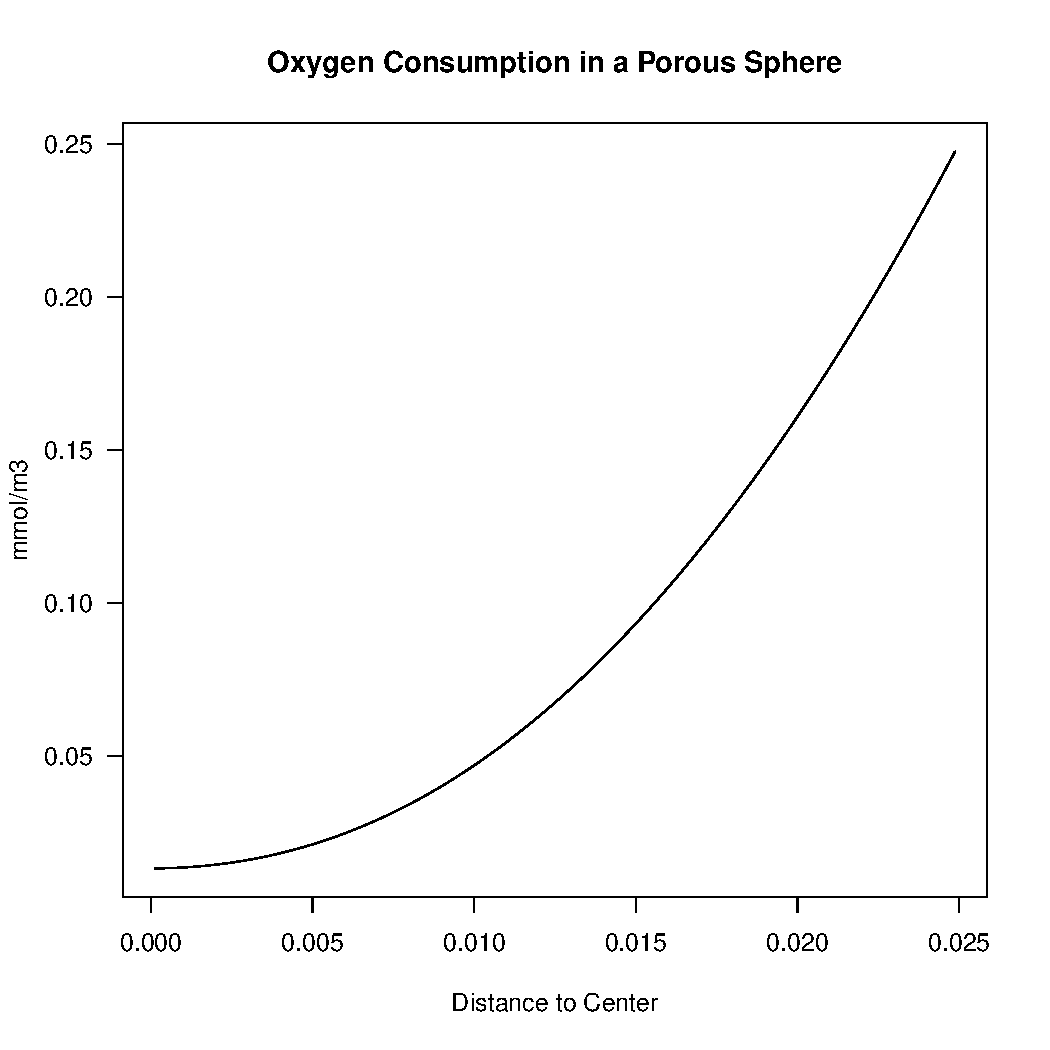
\includegraphics[width=\maxwidth]{figure/plotO2agg-1} 
\end{knitrout}
\end{figure}

The plot shows the oxygen concentration in the particle. The concentration is highest at the surface and decreases as it moves into the particle. The concentration is zero at the center of the particle.

\begin{figure}
\begin{knitrout}
\definecolor{shadecolor}{rgb}{0.969, 0.969, 0.969}\color{fgcolor}
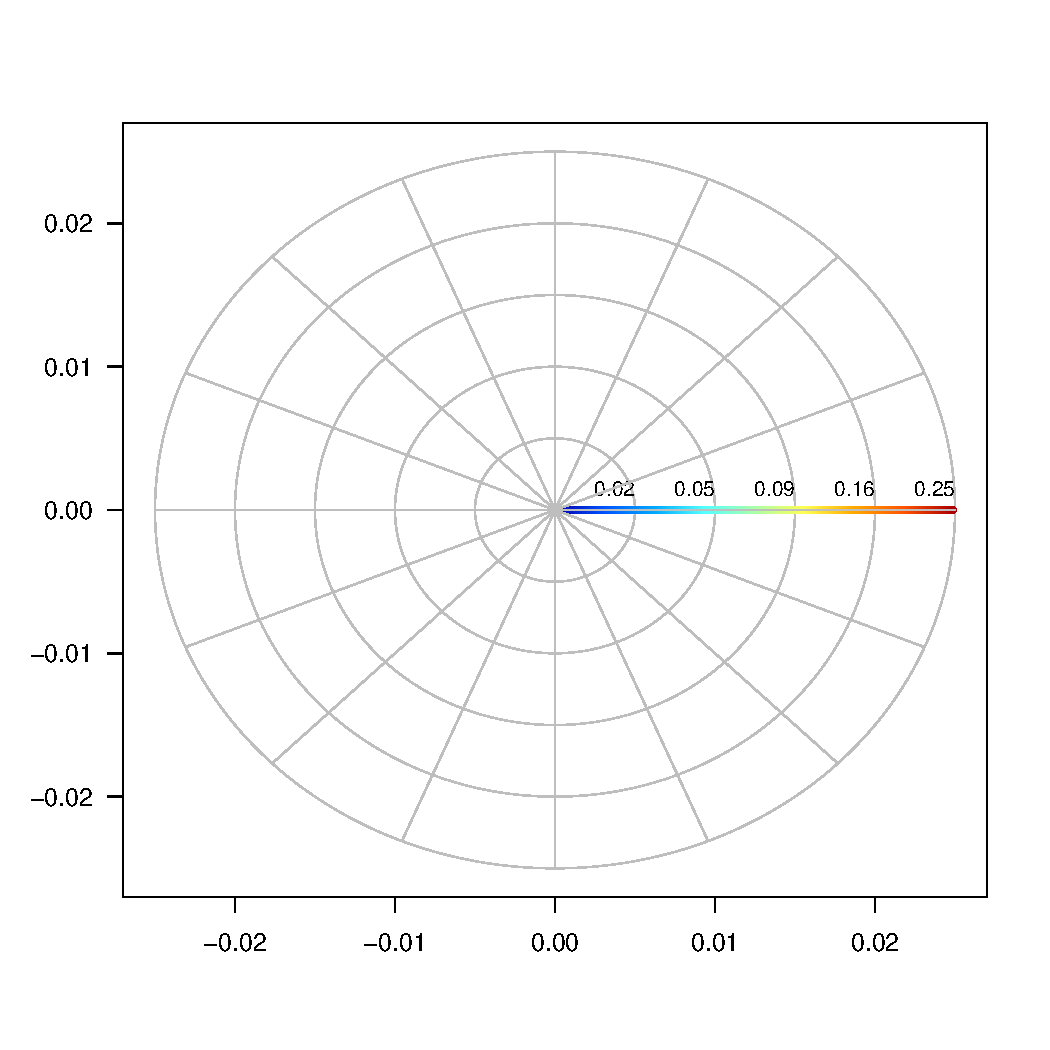
\includegraphics[width=\maxwidth]{figure/circleplot-1} 
\end{knitrout}
\end{figure}

Next steps: figure out how to create a 3D sphere with the oxygen concentration changes as we enter the sphere... 






\section{2D Examples}

Modeling vehicle pollution from cars on a freeway that does in a west to east direction, while pollution moved in a north to south direction. The cars are pollution makers, and the wind is the advection term. The diffusion term is the natural spread of the pollution. The reaction term is the removal of pollution from the air. We'll model this as a steady state, where $\frac{\partial C}{\partial t} = 0$.





Where $\nu_x$  is the velocity in the x direction, $\nu_y$ is the velocity in the y direction, $D$ is the diffusion coefficient, and $R$ is the reaction term.



\begin{equation}
\frac{\partial C}{\partial t} + u \frac{\partial C}{\partial x} + v \frac{\partial C}{\partial y} = D \left( \frac{\partial^2 C}{\partial x^2} + \frac{\partial^2 C}{\partial y^2} \right) - R
\end{equation}

OR? with C as a fuction of y would be better!
\begin{comment}
\begin{equation}
 \frac{\partial C}{\partial y} = \left D \left( \frac{\partial^2 C}{\partial x^2} + \frac{\partial^2 C}{\partial y^2} \right) - R - \nu_x \frac{\partial C}{\partial x} \right \cdot \frac{1}{\nu_y}
\end{equation}
\end{comment}
Not working yet!

\begin{knitrout}
\definecolor{shadecolor}{rgb}{0.969, 0.969, 0.969}\color{fgcolor}\begin{kframe}
\begin{alltt}
\hlcom{# Create a function to model the pollution}

\hlstd{Pollution.Model} \hlkwb{<-} \hlkwa{function}\hlstd{(}\hlkwc{time}\hlstd{,} \hlkwc{C}\hlstd{,} \hlkwc{pars}\hlstd{) \{}
  \hlstd{tran} \hlkwb{<-} \hlkwd{tran.2D}\hlstd{(}\hlkwc{C} \hlstd{= C,} \hlkwc{C.down} \hlstd{= C.ow,} \hlkwc{D} \hlstd{= D.grid,}
          \hlkwc{A}\hlstd{=A.grid,} \hlkwc{VF} \hlstd{= por.grid,} \hlkwc{dx} \hlstd{= grid)}
    \hlstd{reac} \hlkwb{<-} \hlopt{-} \hlstd{R} \hlopt{*} \hlstd{(C} \hlopt{/}\hlstd{(Ks} \hlopt{+} \hlstd{C))}
    \hlkwd{return}\hlstd{(}\hlkwd{list}\hlstd{(}\hlkwc{dCdt}\hlstd{= tran}\hlopt{$}\hlstd{dC} \hlopt{+} \hlstd{reac,} \hlkwc{reac} \hlstd{= reac,}
                \hlkwc{flux.up}\hlstd{=tran}\hlopt{$}\hlstd{flux.up,} \hlkwc{flux.down}\hlstd{=tran}\hlopt{$}\hlstd{flux.down))}
\hlstd{\}}

\hlcom{# Create a 2D grid}

\hlstd{grid} \hlkwb{<-} \hlkwd{expand.grid}\hlstd{(}\hlkwc{x} \hlstd{=} \hlkwd{seq}\hlstd{(}\hlnum{0}\hlstd{,} \hlnum{100}\hlstd{,} \hlkwc{length} \hlstd{=} \hlnum{100}\hlstd{),}
                    \hlkwc{y} \hlstd{=} \hlkwd{seq}\hlstd{(}\hlnum{0}\hlstd{,} \hlnum{100}\hlstd{,} \hlkwc{length} \hlstd{=} \hlnum{100}\hlstd{))}

\hlcom{# Define Initial Conditions}
\hlopt{???}

\hlcom{# Create a 2D model}

\hlstd{Pollution.2D} \hlkwb{<-} \hlkwd{steady.2D}\hlstd{(}\hlkwc{y} \hlstd{=} \hlkwd{runif}\hlstd{(}\hlkwd{nrow}\hlstd{(grid)),} \hlkwc{func}\hlstd{=Pollution.Model,}
                    \hlkwc{nspec}\hlstd{=}\hlnum{1}\hlstd{,} \hlkwc{positive}\hlstd{=}\hlnum{TRUE}\hlstd{,} \hlkwc{atol} \hlstd{=} \hlnum{1e-10}\hlstd{)}


\hlcom{# Plot the 2D model}

\hlkwd{plot}\hlstd{(Pollution.2D,} \hlkwc{grid} \hlstd{= grid,} \hlkwc{xlab} \hlstd{=} \hlstr{"Distance to Center"}\hlstd{,} \hlkwc{ylab} \hlstd{=} \hlstr{"mmol/m3"}\hlstd{,}
     \hlkwc{las}\hlstd{=}\hlnum{1}\hlstd{,} \hlkwc{main}\hlstd{=}\hlstr{"Pollution in a 2D Grid"}\hlstd{)}
\end{alltt}
\end{kframe}
\end{knitrout}






\section{3D Examples}

\section{Conclusion}



\newpage

\section{References}

% bibiliography section here-------------------------------------------
%\clearpage

\url{https://en.wikipedia.org/wiki/Convection%E2%80%93diffusion_equation}



\bibliographystyle{apalike}
%\renewcommand\bibname{References}{}
\bibliography{/home/mwl04747/RTricks/references}%	\addcontentsline{toc}{chapter}{References}


\end{document}
